This chapter discusses the performance level of a single ipvs load balancer.
First the author investigated general characteristics of a single load balancer using physical servers in on-premise data center and compared performance level with existing iptables DNAT and nginx as a load balancer within a 1Gbps network environment.
Then the author also carried out the performance measurement in GCP and AWS to show that the containerized ipvs load balancer is runnable and has the same characteristics in the cloud environment.
Furthermore, experiment was extended into the 10Gbps network environment to investigate the performance limitations of the proposed load balancer and to explore methods to improve them.
The following sections explain these in further detail.

\section{L3DSR}

\begin{figure}[h]
  \centering
  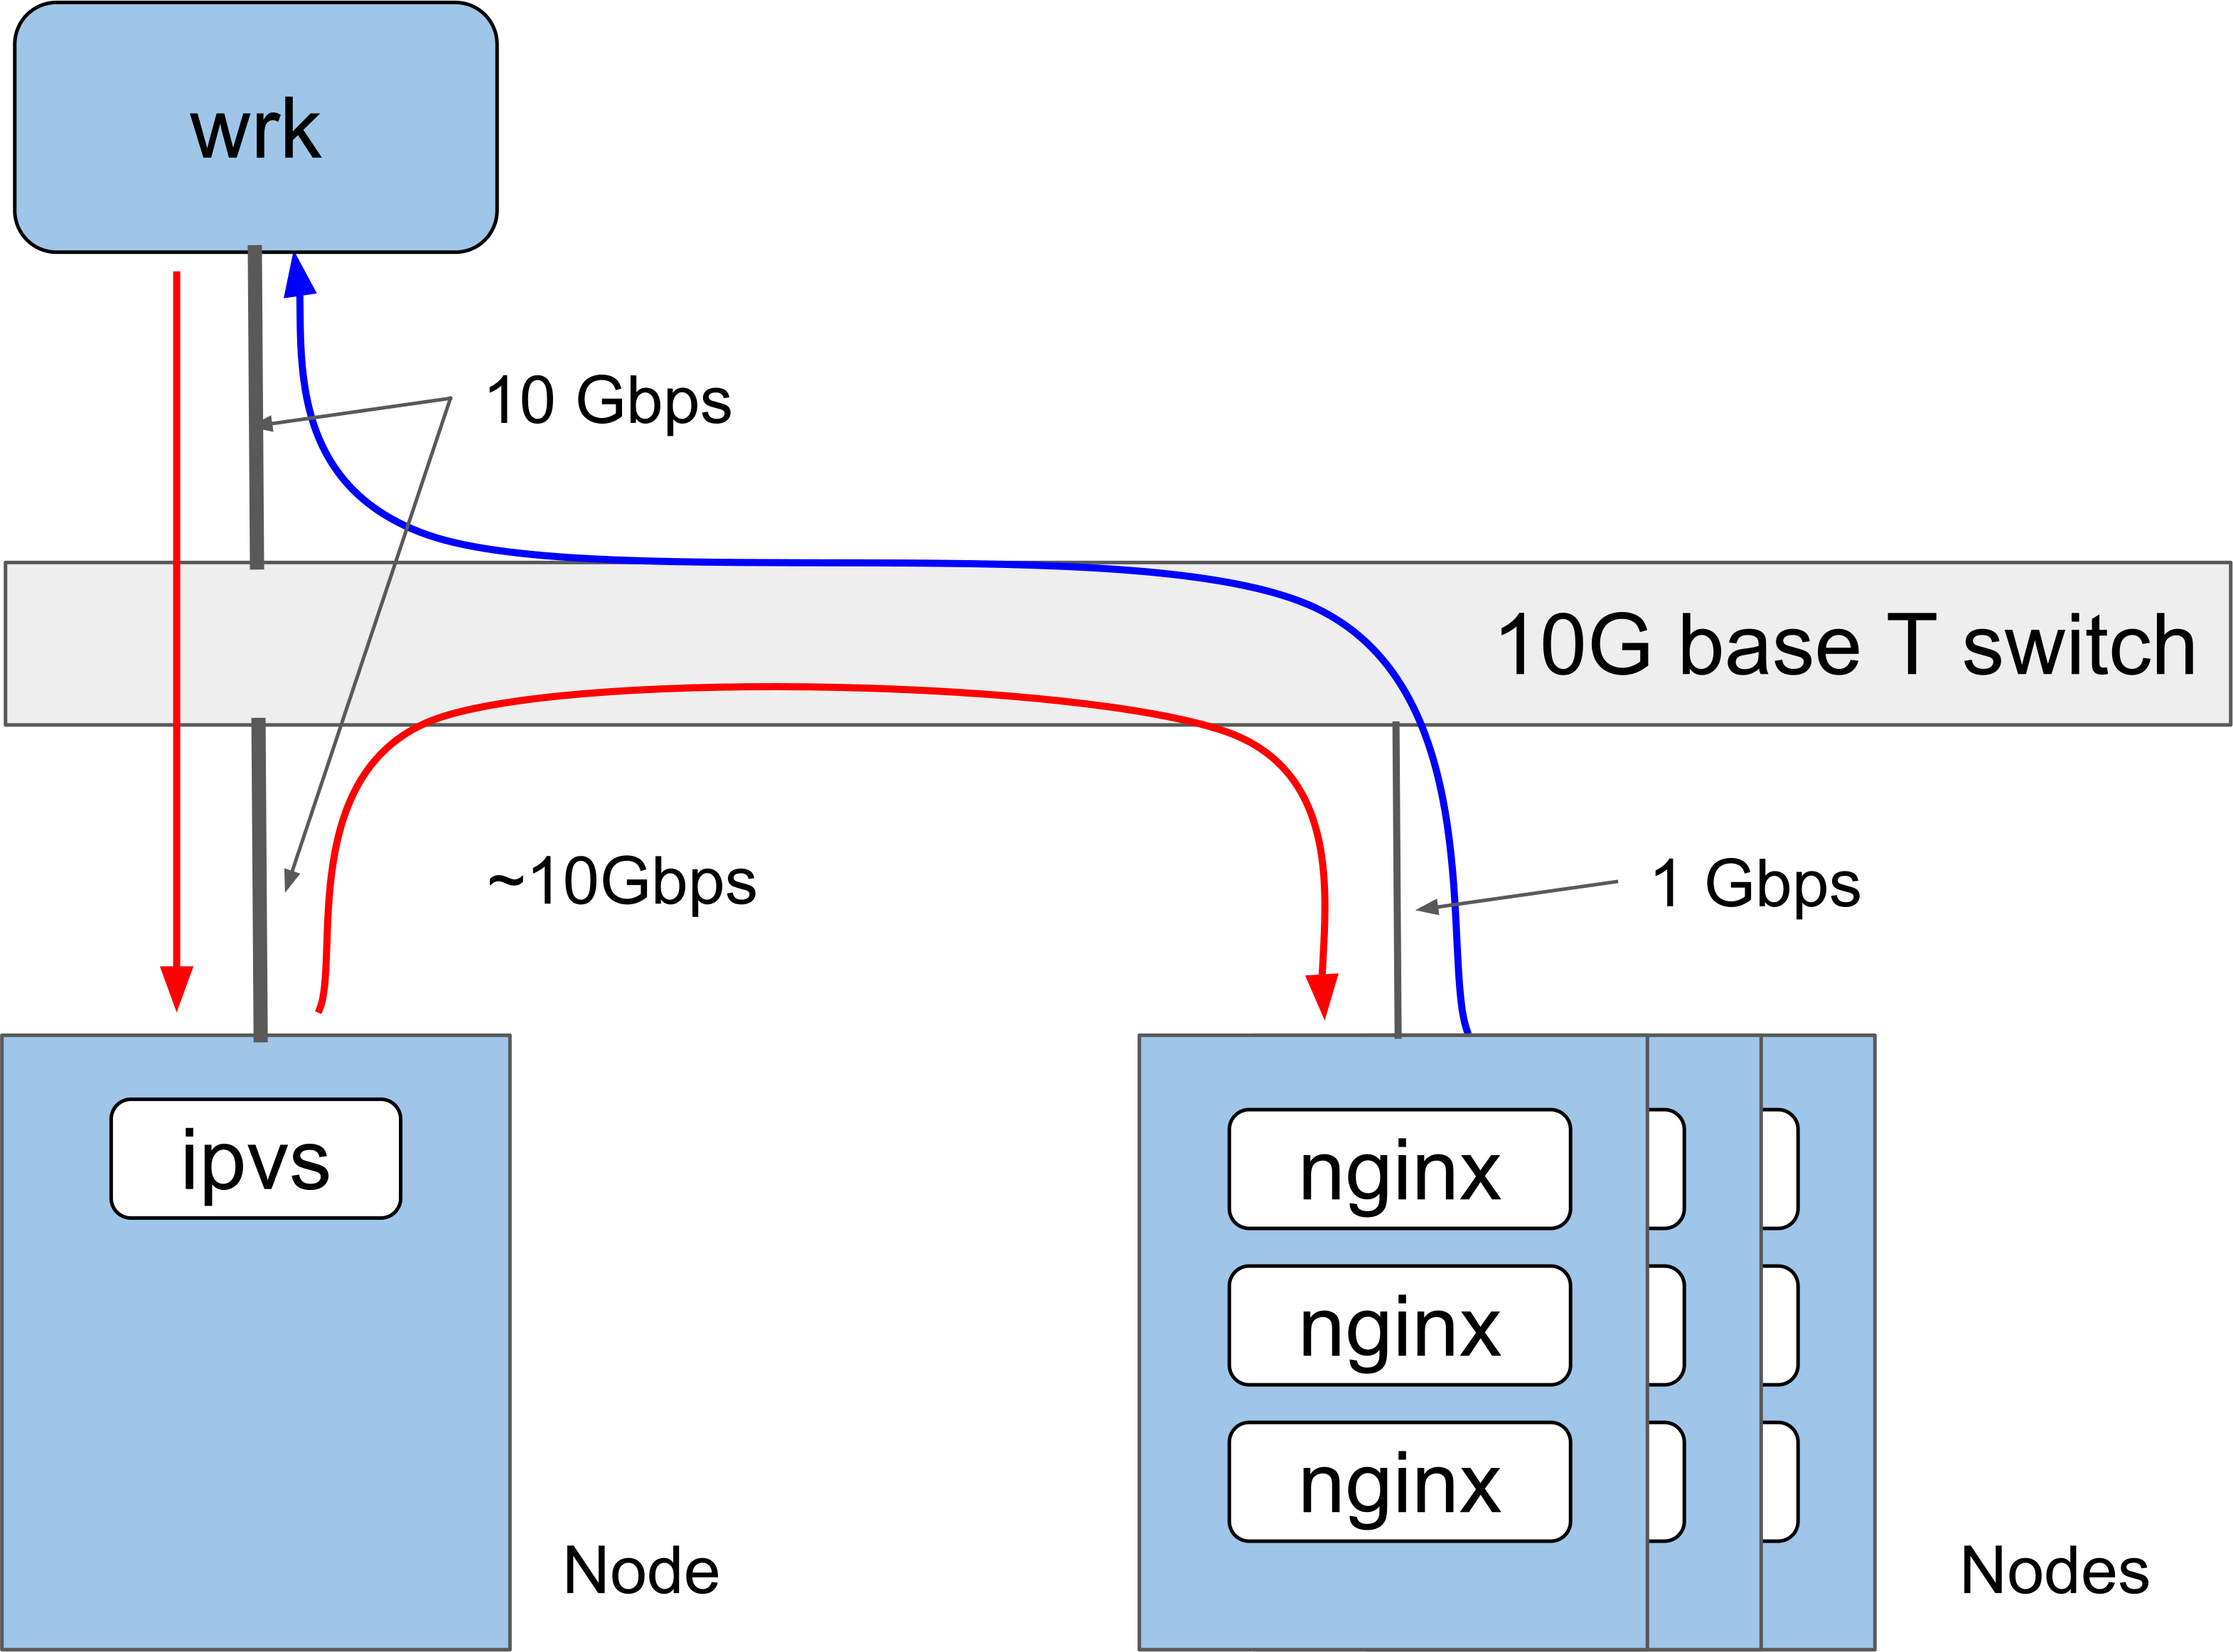
\includegraphics[width=0.8\columnwidth]{Figs/bench_10g_l3dsr}
  \caption{Physical configuration for L3DSR experiment.}
  \label{fig:bench_10g_l3dsr}
\end{figure}

\begin{figure}[h]
  \centering
  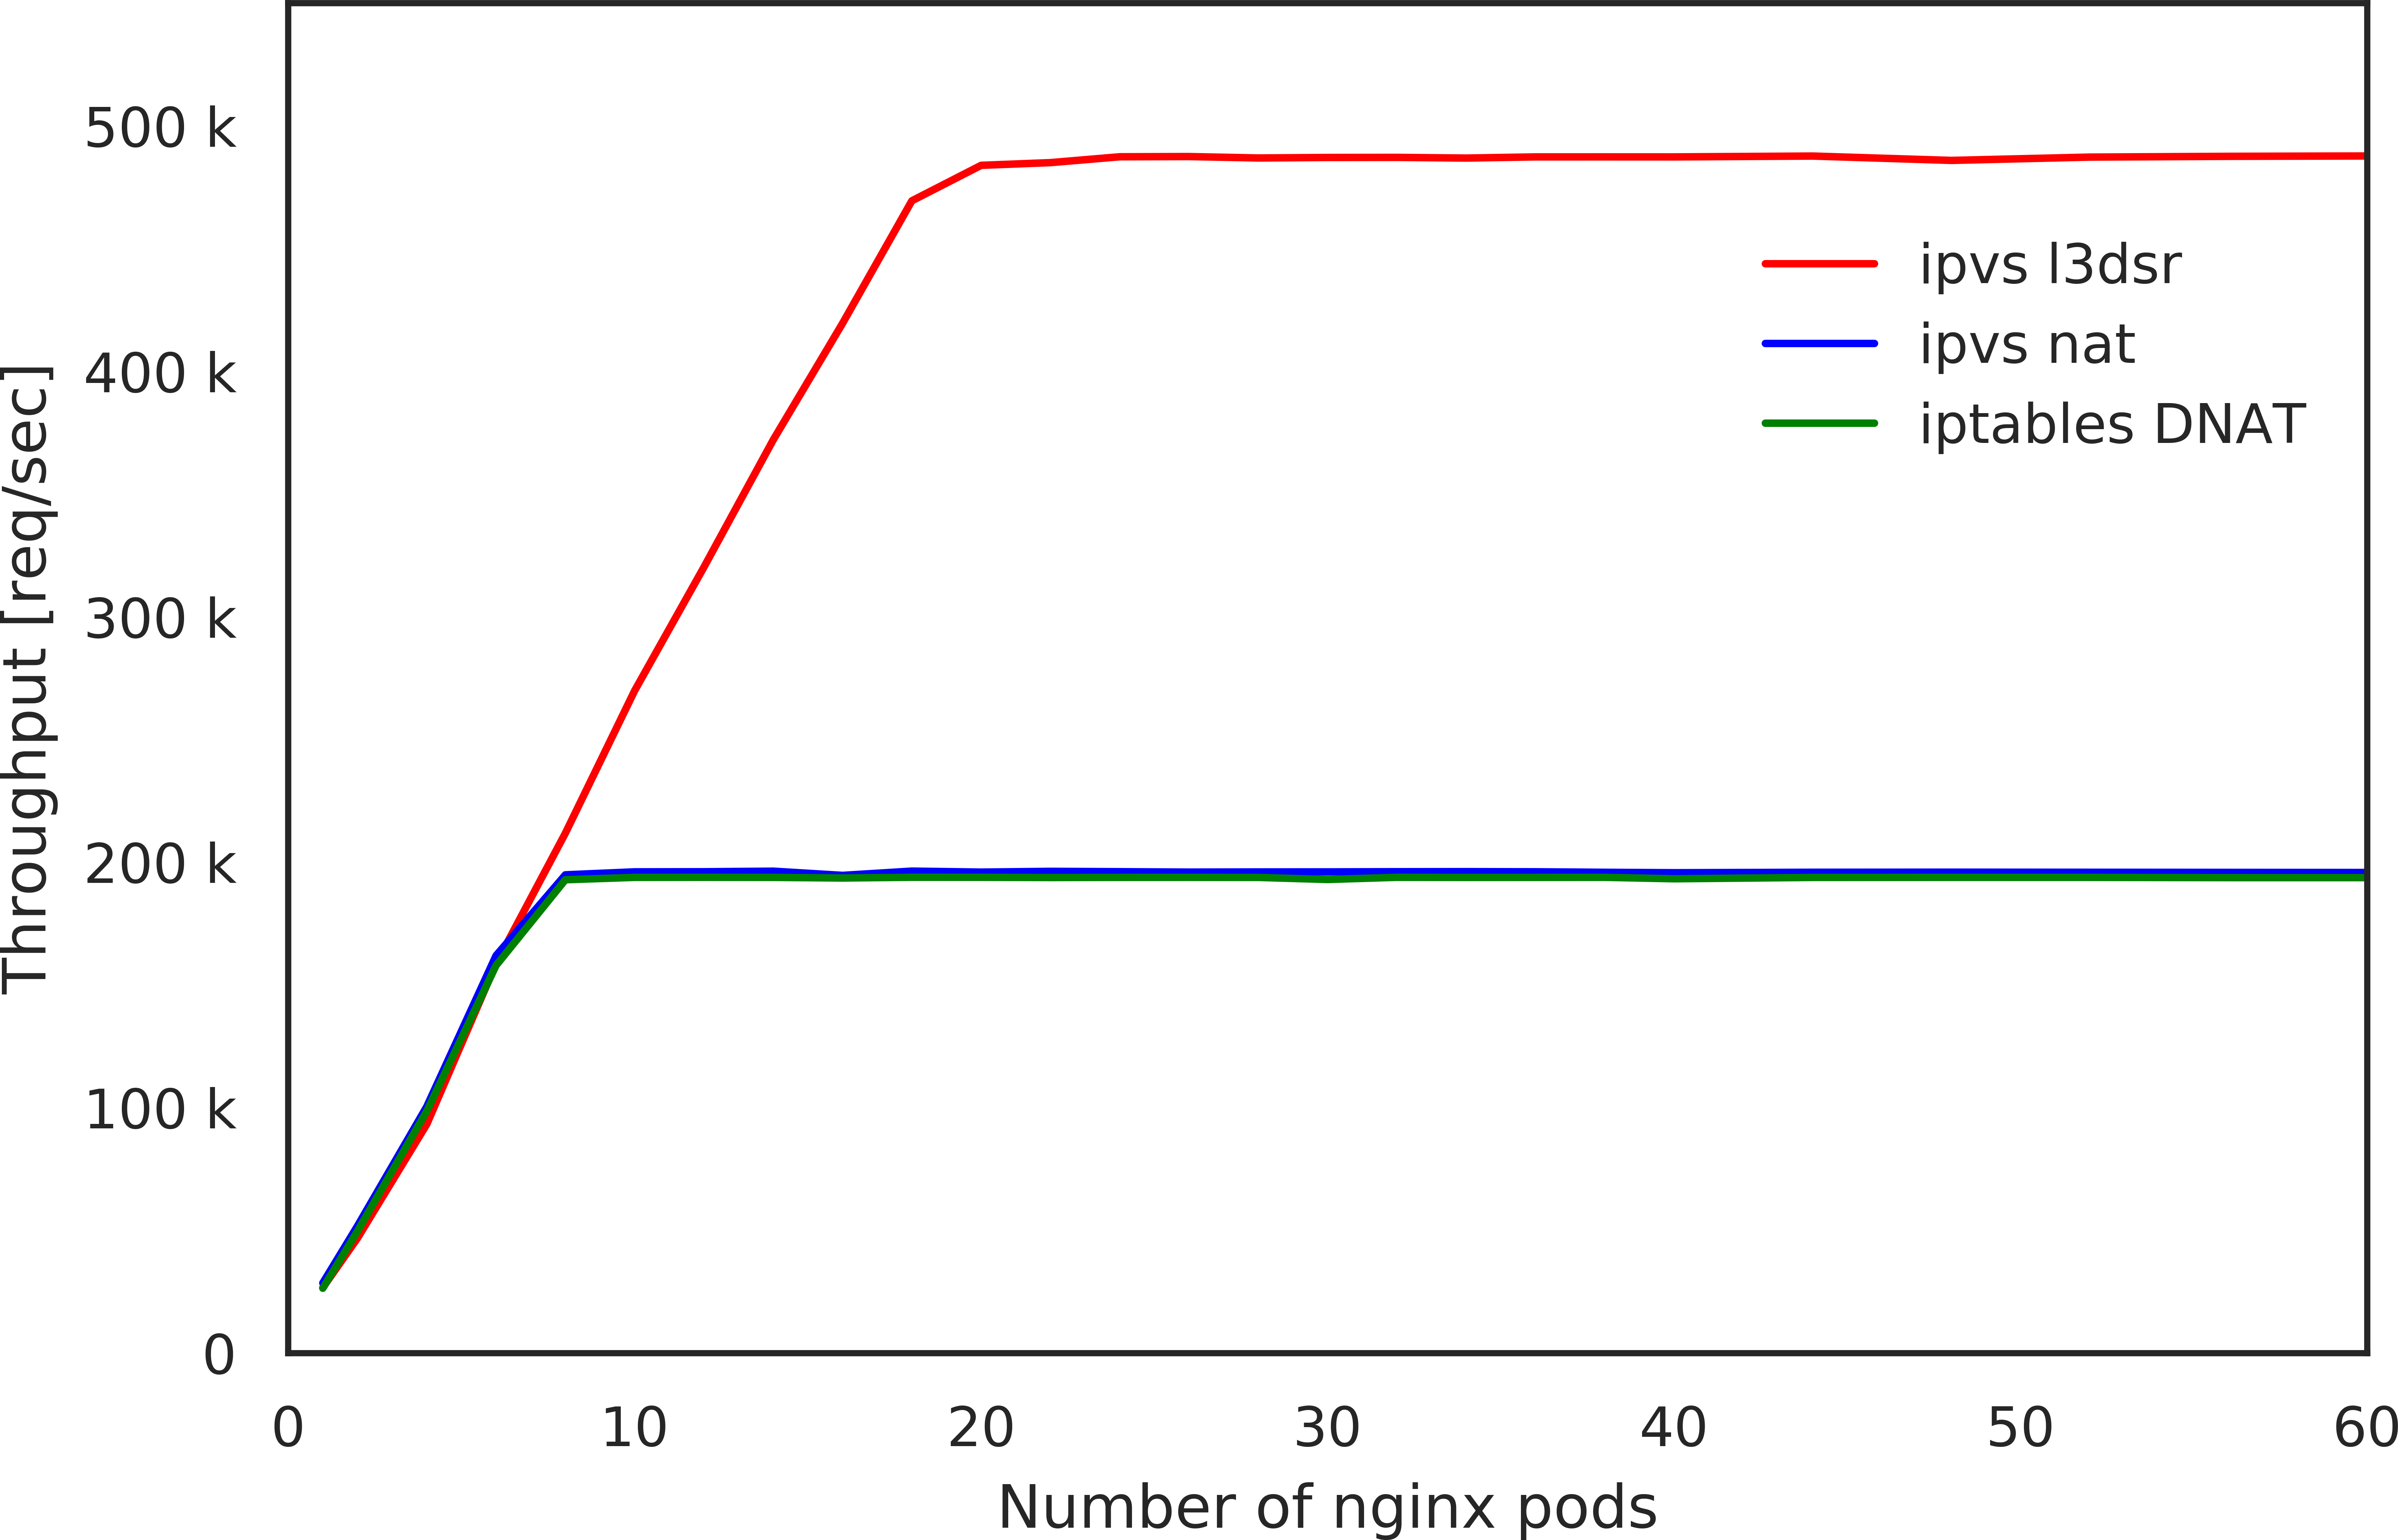
\includegraphics[width=0.8\columnwidth]{Figs/ipvs_l3dsr_1g.png}
  \caption{Throughput of ipvs l3dsr @1Gbps.}
  \label{fig:ipvs_l3dsr_1g.png}
\end{figure}

\section{Load balancer for 10Gbps environment}

\begin{figure}[h]
  \centering
  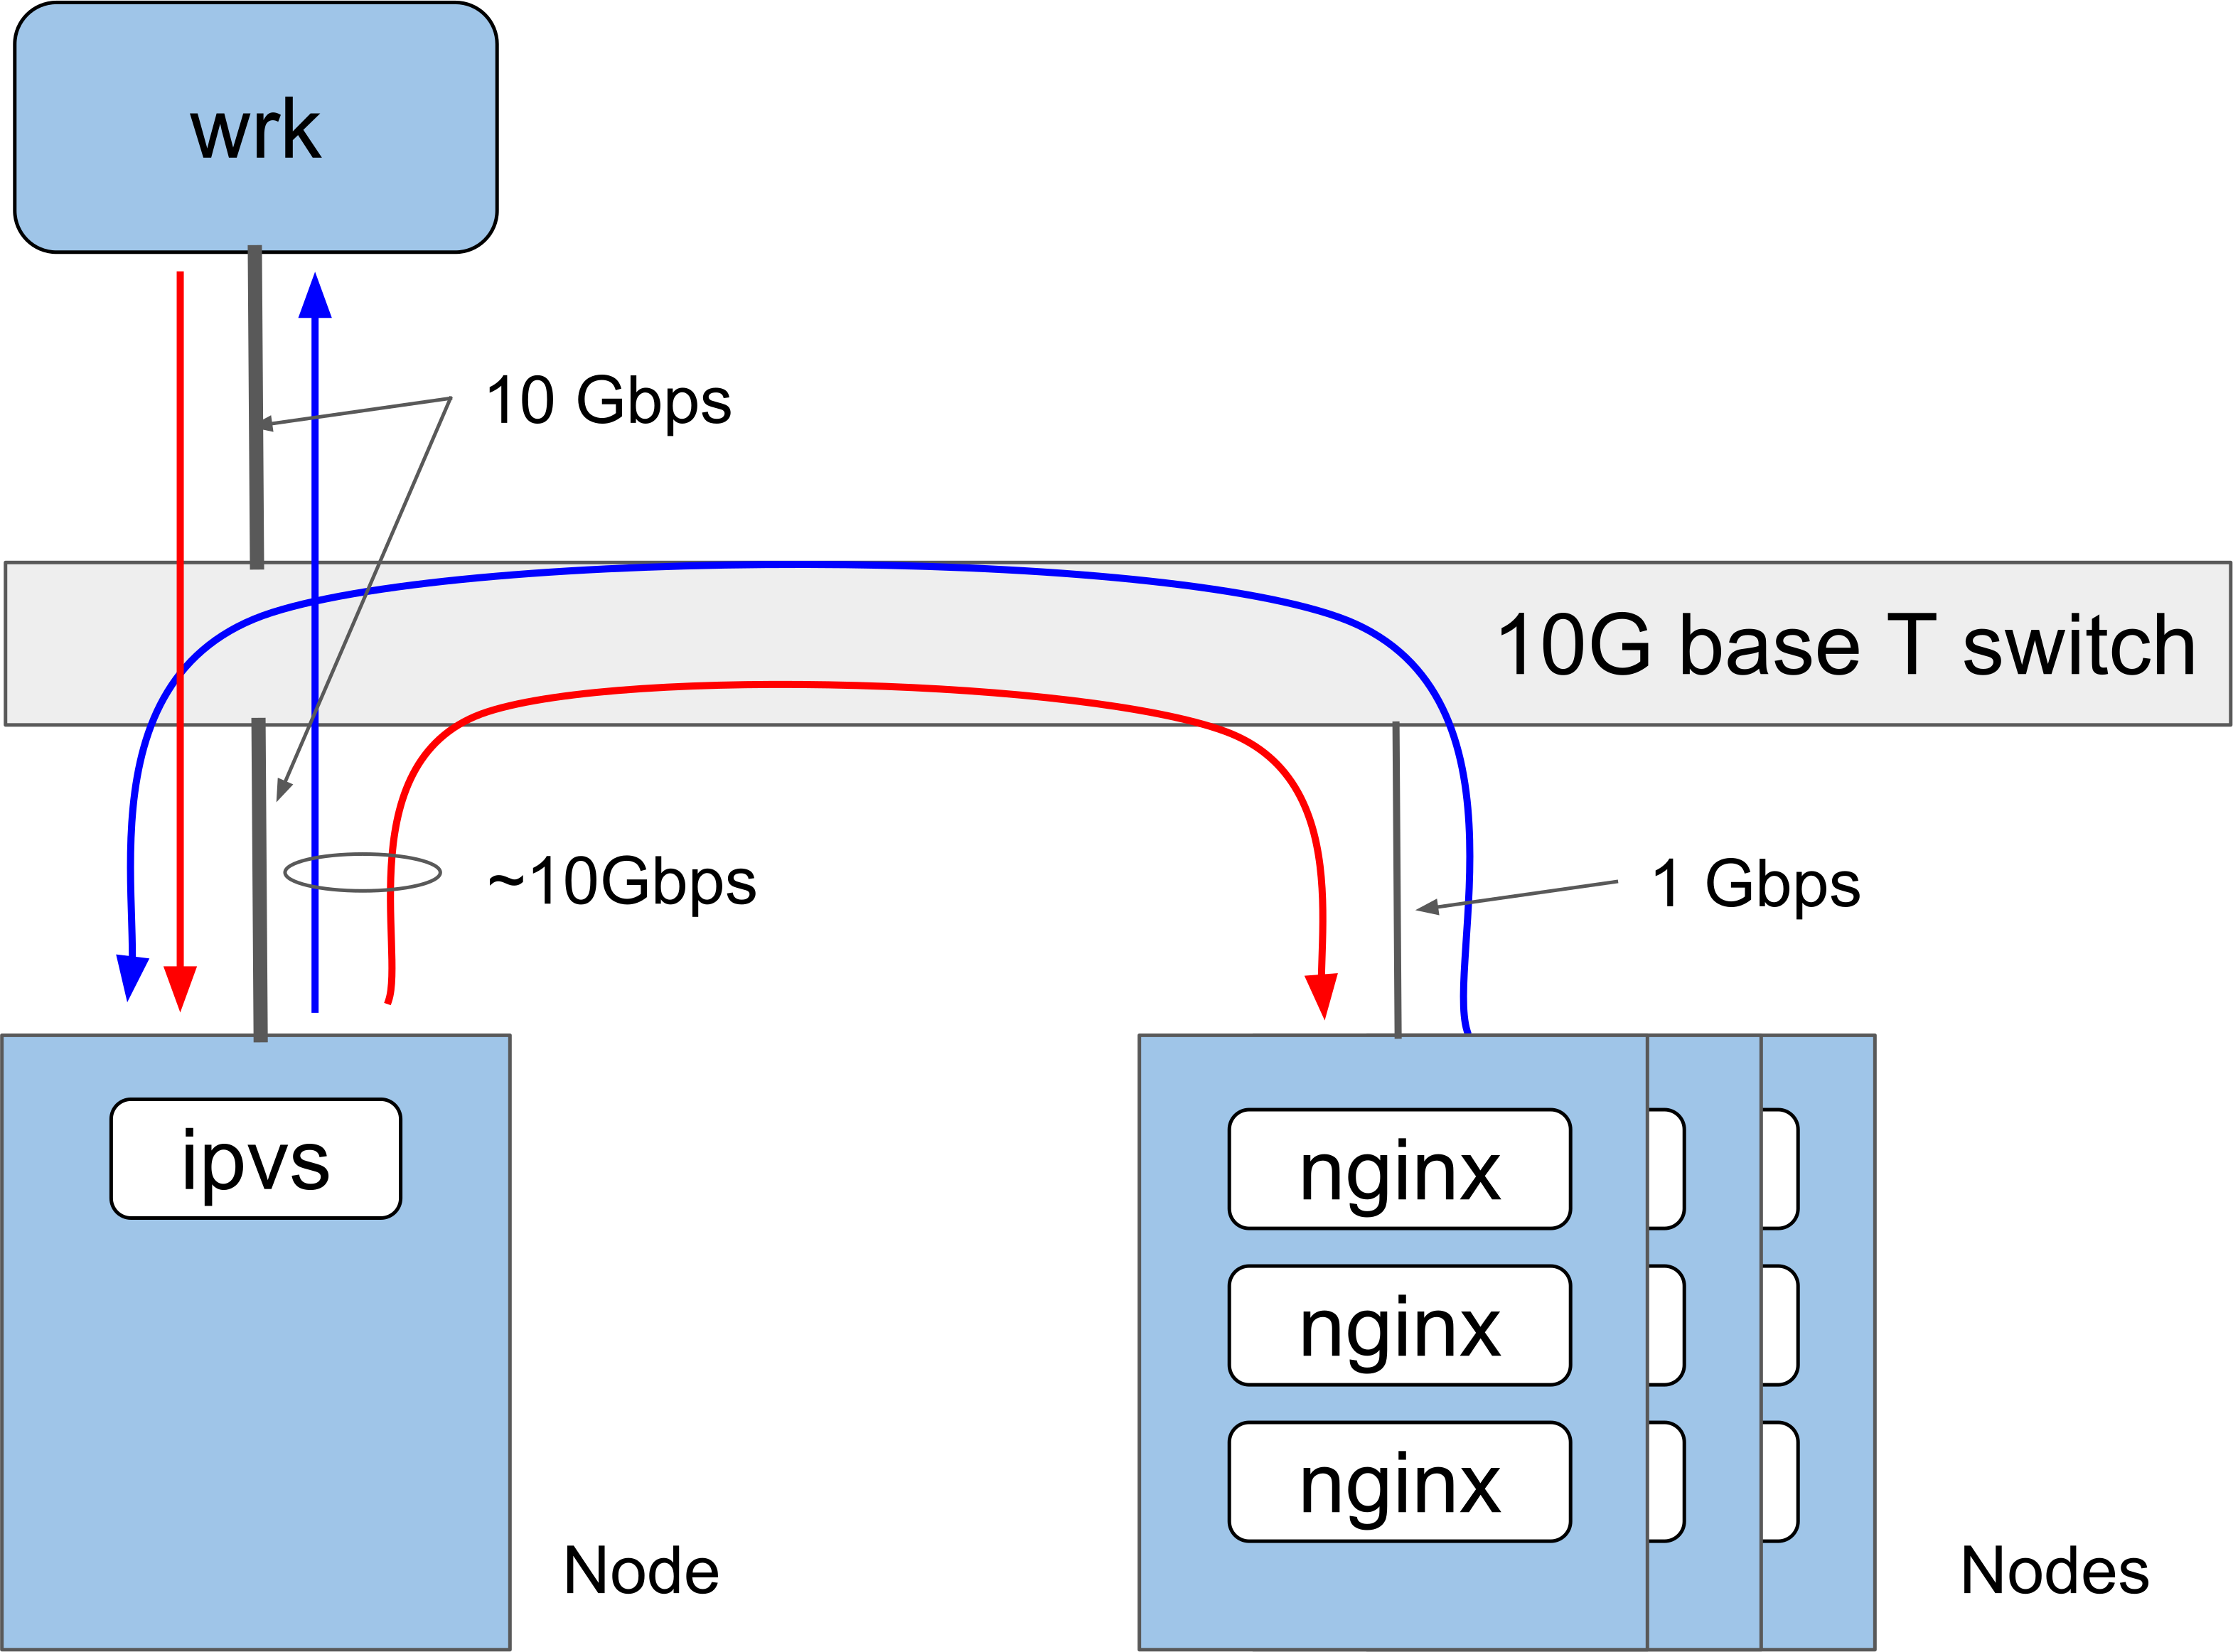
\includegraphics[width=0.8\columnwidth]{Figs/bench_10g}
  \caption{Physical configuration for 10Gbps measurement.}
  \label{fig:bench_10g}
\end{figure}

\begin{figure}[t]
  \centering
  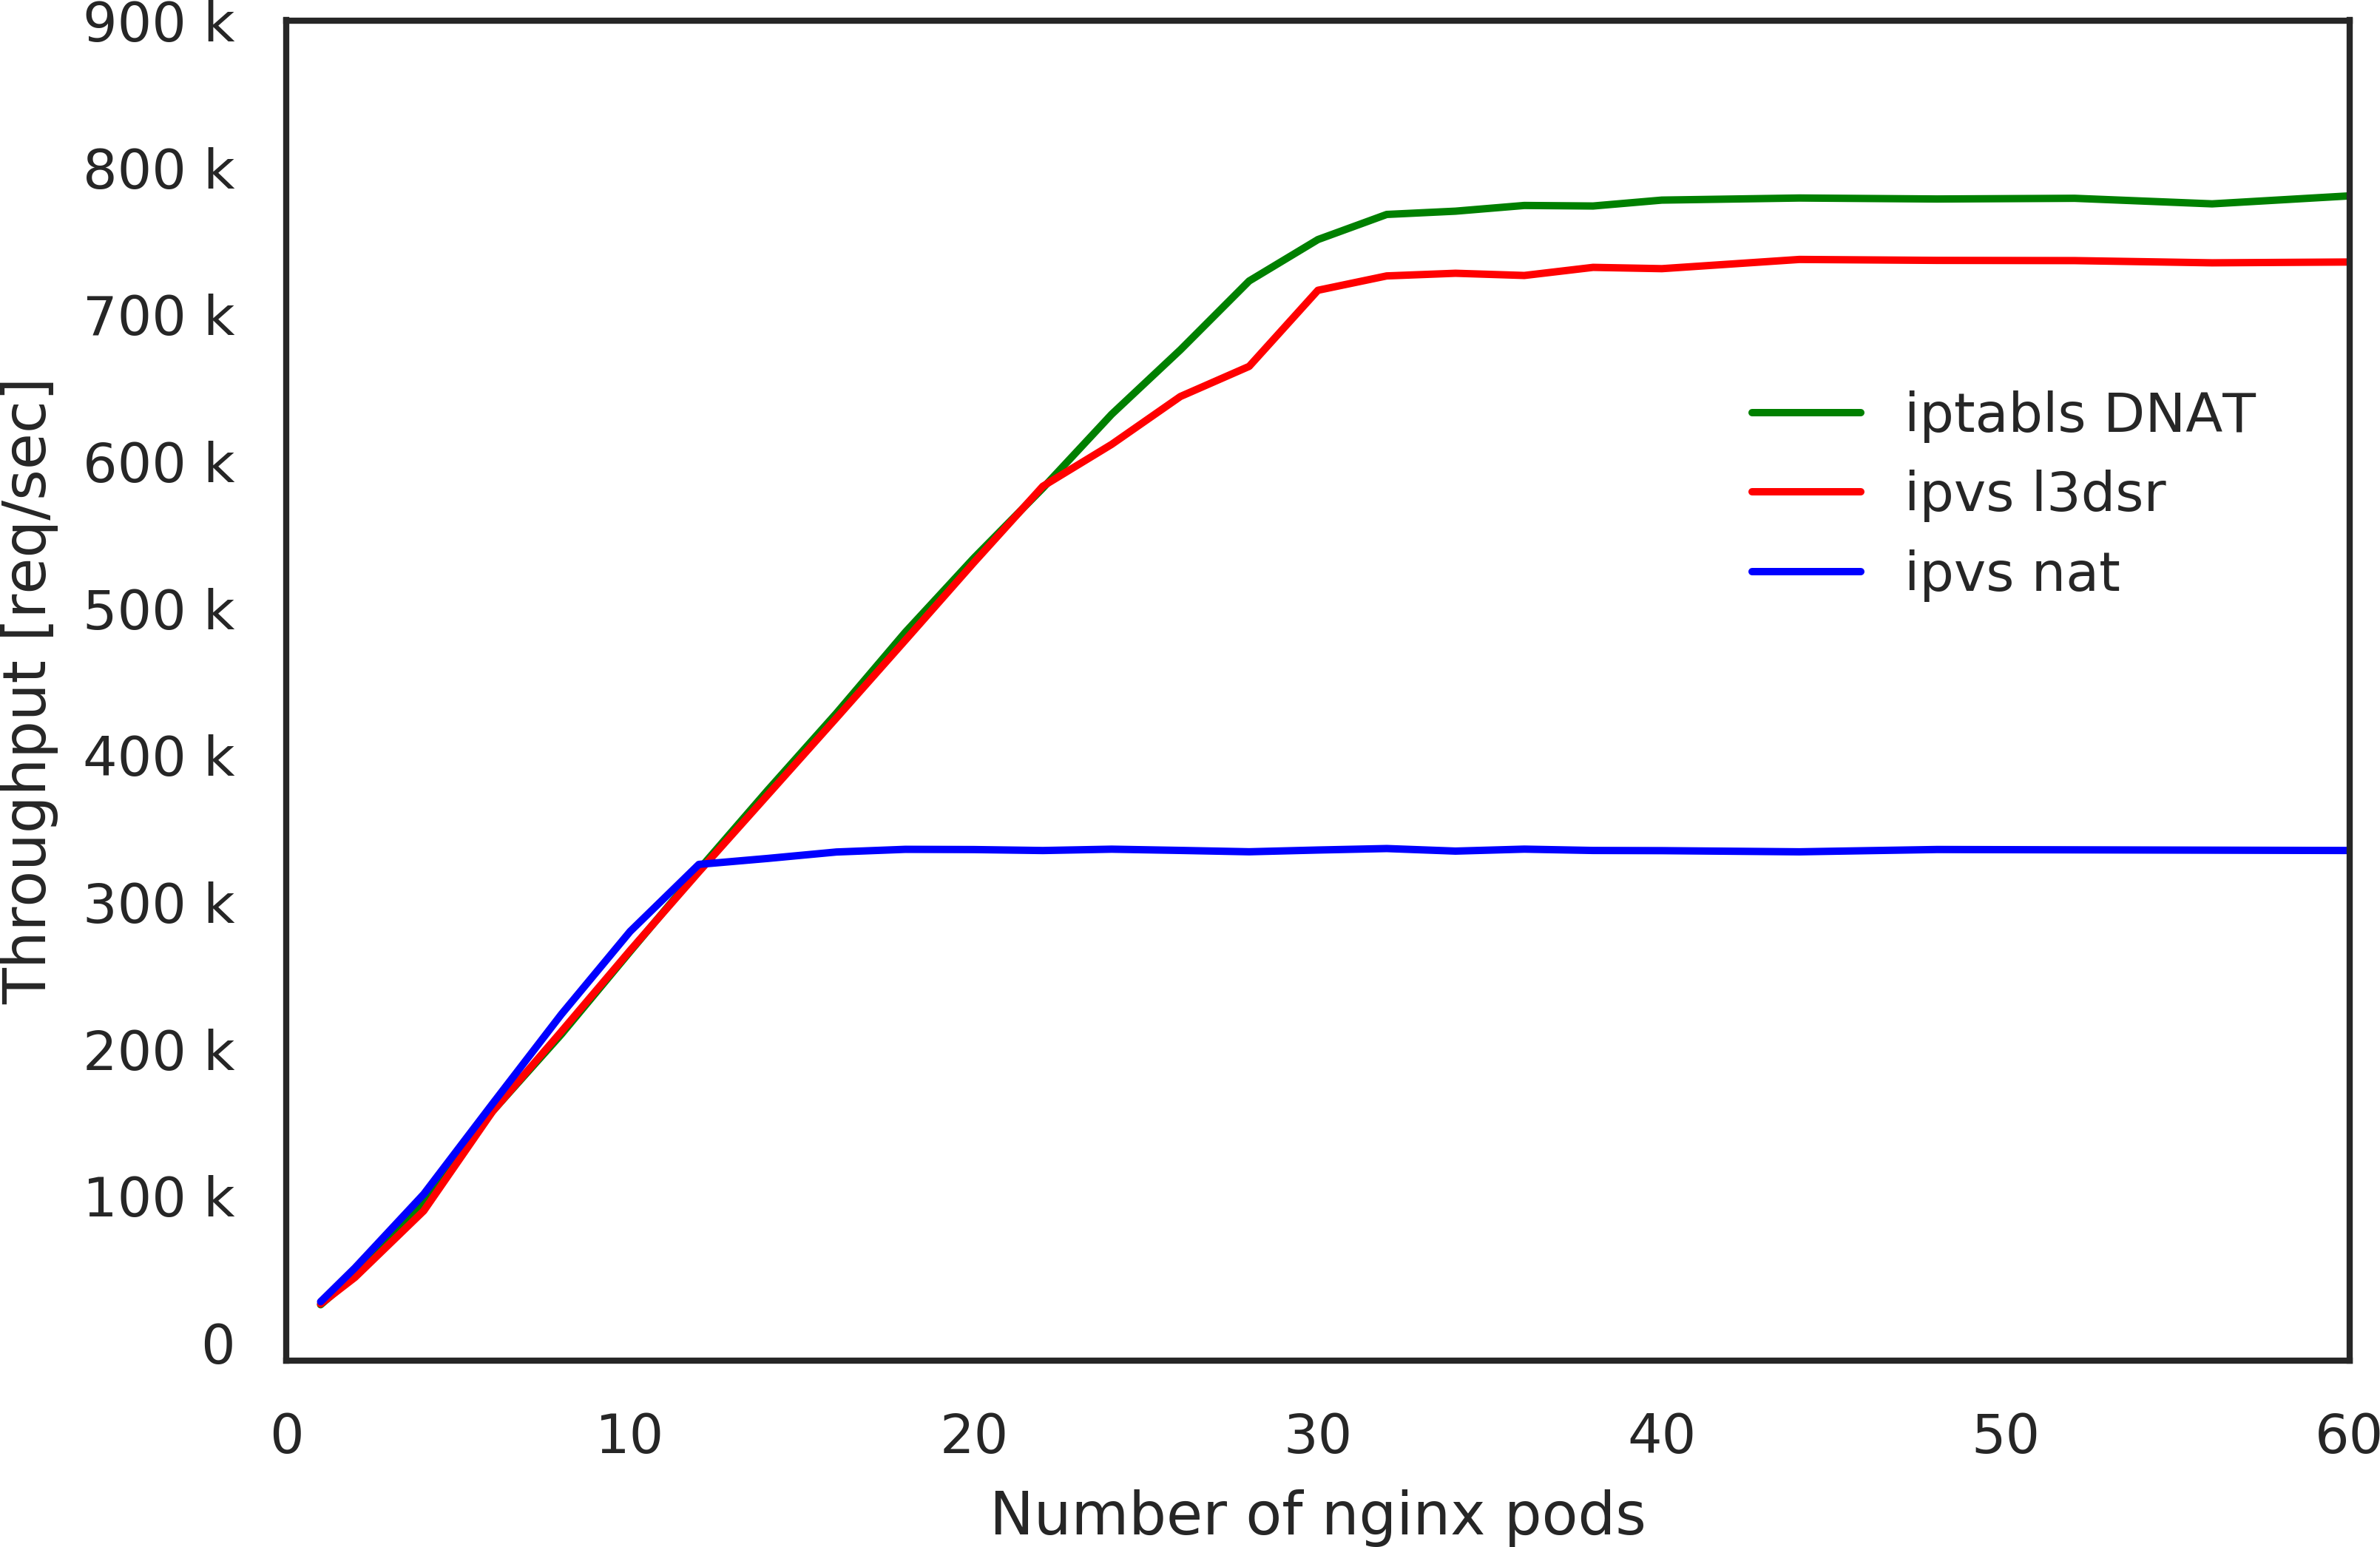
\includegraphics[width=0.8\columnwidth]{Figs/ipvs_l3dsr_10g.png}
  \caption{Throughput of ipvs l3dsr @10Gbps.}
  \label{fig:ipvs_l3dsr_10g.png}
\end{figure}

\section{XDP load balancer}

\section{Summary}



